\begin{enumerate}[label=\thesection.\arabic*,ref=\thesection.\theenumi]
\numberwithin{equation}{enumi}
\numberwithin{figure}{enumi}
\numberwithin{table}{enumi}

\item 
\item 
\item 
\label{chapters/11/10/3/4}
\iffalse
\documentclass[12pt]{article}
\usepackage{graphicx}
\usepackage[none]{hyphenat}
\usepackage{graphicx}
\usepackage{listings}
\usepackage[english]{babel}
\usepackage{graphicx}
\usepackage{caption} 
\usepackage{booktabs}
\usepackage{array}
\usepackage{amssymb} % for \because
\usepackage{amsmath}   % for having text in math mode
\usepackage{extarrows} % for Row operations arrows
\usepackage{listings}
\lstset{
  frame=single,
  breaklines=true
}
\usepackage{hyperref}
  
%Following 2 lines were added to remove the blank page at the beginning
\usepackage{atbegshi}% http://ctan.org/pkg/atbegshi
\AtBeginDocument{\AtBeginShipoutNext{\AtBeginShipoutDiscard}}


%New macro definitions
\newcommand{\mydet}[1]{\ensuremath{\begin{vmatrix}#1\end{vmatrix}}}
\providecommand{\brak}[1]{\ensuremath{\left(#1\right)}}
\providecommand{\norm}[1]{\left\lVert#1\right\rVert}
\newcommand{\solution}{\noindent \textbf{Solution: }}
\newcommand{\myvec}[1]{\ensuremath{\begin{pmatrix}#1\end{pmatrix}}}
\providecommand{\abs}[1]{\left\vert#1\right\vert}
\let\vec\mathbf

\begin{document}

\begin{center}
\title{\textbf{Equation  of Line}}
\date{\vspace{-5ex}} %Not to print date automatically
\maketitle
\end{center}
\setcounter{page}{1}

\section{11$^{th}$ Maths - Chapter 10}
This is Problem-4 from Exercise 10.3
\begin{enumerate}
		\fi
	\\
\solution 
\begin{enumerate}
\item The equation of the line is $12\brak{x+6} = 5\brak{y-2}$. Rearranging the equation, 
\begin{align}
12x-5y = -10-72 \\
12x-5y = -82
\end{align}

This can be equated to

\begin{align}
	\label{eq:11/10/3/4/2Dline}
	\vec{n}^\top\vec{x} = c 
\end{align}
\begin{align}
	\text{ where }
		\vec{n} = \myvec{
	  12 \\
	  -5 
	  } ,   c = -82 
\end{align}
		We need to compute the distance from a point $\vec{P}\myvec{-1 \\ 1}$ to the line. 
Without loss of generality, let $\vec{A}$ be the foot of the perpendicular from $\vec{P}$ to the line in Equation \eqref{eq:11/10/3/4/2Dline}. 
The equation of the normal to Equation \eqref{eq:11/10/3/4/2Dline} can then be expressed as 

\begin{align}
	\label{eq:11/10/3/4/dir_line_normal_dist}
	\vec{x} &= \vec{A} + \lambda \vec{n}
	\\
	\implies 
	\label{eq:11/10/3/4/dir_line_normal_dist_pa}
	\vec{P}- \vec{A} &=  \lambda \vec{n}
\end{align}

$\because \vec{P}$ lies on 
		\eqref{eq:11/10/3/4/dir_line_normal_dist}.
From the above, the desired distance can be expressed as 

\begin{align}
	\label{eq:11/10/3/4/dir_line_normal_dist_pa_d}
d = 	\norm{\vec{P}- \vec{A}}= \abs{\lambda} \norm{\vec{n}}
\end{align}

From 
	\eqref{eq:11/10/3/4/dir_line_normal_dist_pa},

\begin{align}
	\vec{n}^{\top}
	\brak{\vec{P}- \vec{A}} &=  \lambda \vec{n}^{\top}\vec{n} = \lambda\norm{\vec{n}}^2
	\\
	\implies \abs{\lambda}&= \frac{\abs{\vec{n}^{\top}
	\brak{\vec{P}- \vec{A}}}}{\norm{\vec{n}}^2} 
\end{align}

Substituting the above in \eqref{eq:11/10/3/4/dir_line_normal_dist_pa_d} and using the fact that

\begin{align}
   \vec{n}^{\top}\vec{A} = c
\end{align}

from 	\eqref{eq:11/10/3/4/2Dline}, yields 

\begin{align}
	\label{eq:11/10/3/4/line_dist_2d}
	d = \frac{\abs{   \vec{n}^{\top}\vec{P}-c }}{\norm{\vec{n}}}	
\end{align}

\begin{align}
	= \frac{\abs{  \myvec{12 & -5 }\myvec{-1 \\ 1}-\brak{-82} }}{\sqrt{12^2+\brak{-5}^2}} \\	
	= \frac{\abs{  -17 + 82 }}{\sqrt{169}}	
	= \frac{\abs{65 }}{13}
	= 5 \text{ units }
\end{align}
\item The foot of the perpendicular from $\vec{P}\myvec{-1 \\ 1}$ to line in \eqref{eq:11/10/3/4/2Dline} is expressed as
\begin{align}
	\label{eq:11/10/3/4/foot_of_perpendicular}
	\myvec{\vec{m} & \vec{n}}^\top\vec{A} &= 
	   \myvec{
              \vec{m}^\top\vec{P}\\
	      c
	      }
\end{align}
where $\vec{m}$ is the direction vector of the given line
\begin{align}
    \because \vec{n} = \myvec{ 12 \\ -5},   
    \vec{m} = \myvec{ 5 \\ 12} \\ 
	\eqref{eq:11/10/3/4/foot_of_perpendicular} \implies \myvec{5&12 \\ 12 & -5}\vec{A} &= \myvec{\myvec{5 & 12}\myvec{-1 \\ 1}\\ -82} \\
	\label{eq:11/10/3/4/sysEq1}
	\myvec{5&12 \\ 12 & -5}\vec{A} &= \myvec{7 \\ -82} 
\end{align}	
The augmented matrix for the system equations in \eqref{eq:11/10/3/4/sysEq1} is expressed as
\begin{align}
	\myvec{5&12 & \vrule & 7 \\ 12 & -5 & \vrule & -82} 
\end{align}
Performing sequence of row operations to transform into RREF form
\begin{align}
        \xleftrightarrow[]{{R_2\rightarrow R_2-\frac{12}{5}R_1}}  
	\myvec{5&12 & \vrule & 7 \\ 0 & -\frac{169}{5} & \vrule & -\frac{494}{5}} \\
	\xleftrightarrow[{R_1\rightarrow \frac{1}{5}}R_1]{{R_2\rightarrow \frac{-5}{169}R_2}}  
	\myvec{1 & \frac{12}{5} & \vrule & \frac{7}{5} \\ 0 & 1 & \vrule & \frac{38}{13}} \\
	\xleftrightarrow[]{{R_1\rightarrow R_1-\frac{12}{5}R_2}}  
	\myvec{1 & 0 & \vrule & -\frac{73}{13} \\ 0 & 1 & \vrule & \frac{38}{13}} \\
	\vec{A} = \myvec{ -\frac{73}{13} \\ \frac{38}{13} }
\end{align}
\end{enumerate}
The desired line and the perpendicular line from $\vec{P}$ is shown as in Fig. \ref{fig:11/10/3/4/Fig1}
\begin{figure}[!h]
	\begin{center}
		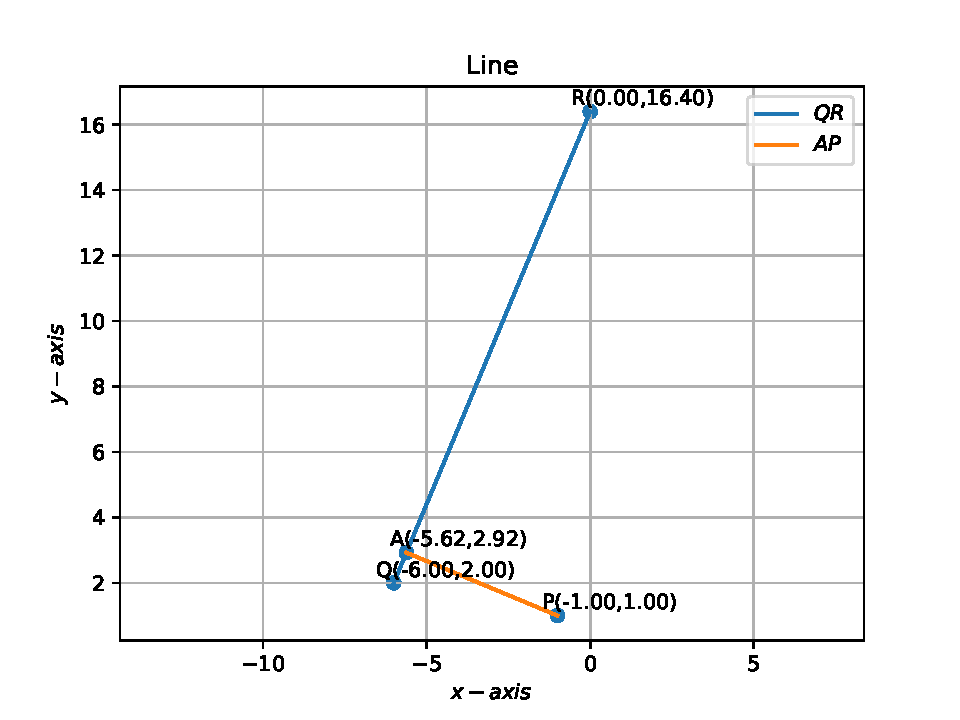
\includegraphics[width=\columnwidth]{chapters/11/10/3/4/figs/problem4.pdf}
	\end{center}
\caption{}
\label{fig:11/10/3/4/Fig1}
\end{figure}

\item Find the points on the x-axis, whose distances from the line $\frac{x}{3}+\frac{y}{4}=1$ are 4 units.
\label{chapters/11/10/3/5}
	\\
	\solution
\iffalse
\documentclass[12pt]{article}
\usepackage{graphicx}
\usepackage{amsmath}
\usepackage{mathtools}
\usepackage{gensymb}
\usepackage{amssymb}

\newcommand{\mydet}[1]{\ensuremath{\begin{vmatrix}#1\end{vmatrix}}}
\providecommand{\brak}[1]{\ensuremath{\left(#1\right)}}
\providecommand{\norm}[1]{\left\lVert#1\right\rVert}
\newcommand{\solution}{\noindent \textbf{Solution: }}
\newcommand{\myvec}[1]{\ensuremath{\begin{pmatrix}#1\end{pmatrix}}}
\providecommand{\abs}[1]{\left\vert#1\right\vert}	
\let\vec\mathbf

\begin{document}
\begin{center}
\textbf\large{CLASS 11 CHAPTER-11 \\ LINES}

\end{center}
\section*{Exercise 10.3}


\solution
\fi
The given line can be expressed as 
\begin{align}
	\vec{n}^{\top}\vec{x}&=c,
	\text{ where }
		\vec{n} &= \myvec{4\\3} , c = 12
\end{align}
The distance formula is given by
\begin{align}
	d = \frac{\abs{\vec{n}^\top\vec{P}-c}}{\norm{\vec{n}}}
\end{align}
Let the desired point be
\begin{align}
	\vec{P} = x\vec{e}_{1} = \myvec{x\\0}
\end{align}
Substituting the values in the distance formula, 
\begin{align}
	d &= \frac{\abs{\vec{n}^\top\vec{P}-c}}{\norm{\vec{n}}}\\
	  &= \frac{\abs{x\vec{n}^\top\vec{e}_{1}-c}}{\norm{\vec{n}}}
	  \\
	  \implies 
	\abs{x\vec{n}^\top\vec{e}_{1}-c} &= d\norm{\vec{n}}
	\\
	\text{or, }	x = \frac{\pm d\norm{\vec{n}}+c}{\vec{n}^\top\vec{e}_{1}}
\end{align}
Since 
\begin{align}
	d &= 4,
\end{align}
substituting numerical values, 
\begin{align}
	x = 8,
	 -2
\end{align}
This is verified in Fig. 
\ref{fig:11/10/3/5/Fig1}.	
\begin{figure}[!h]
	\begin{center} 
	    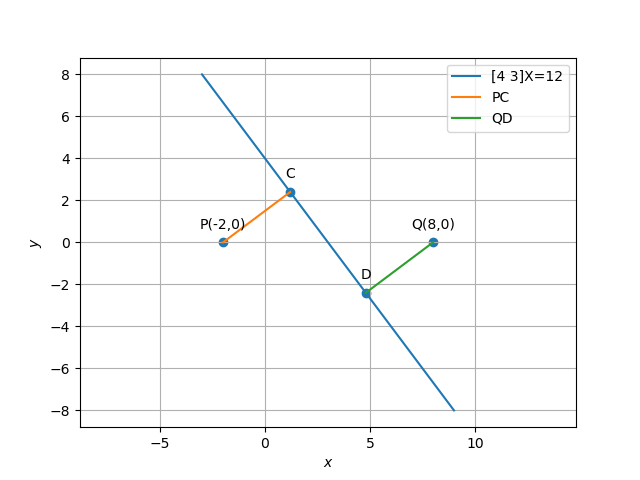
\includegraphics[width=\columnwidth]{chapters/11/10/3/5/figs/line2}
	\end{center}
\caption{}
\label{fig:11/10/3/5/Fig1}
\end{figure}



\item 
\item 
\label{chapters/11/10/3/7}
\iffalse
% #######################################
% ########### FILL THESE IN #############
% #######################################
\def\mytitle{MATRICES}
\def\mykeywords{}
\def\myauthor{GOWTHAMI MANDAVA}
\def\contact{gowthamimandava999@gmail.com}
\def\mymodule{ Future Wireless Communication(FWC22012)}
% #######################################
% #### YOU DON'T NEED TO TOUCH BELOW ####
% #######################################
\newcommand{\myvec}[1]{\ensuremath{\begin{pmatrix}#1\end{pmatrix}}}
\let\vec\mathbf
\providecommand{\pr}[1]{\ensuremath{\Pr\left(#1\right)}}
\providecommand{\qfunc}[1]{\ensuremath{Q\left(#1\right)}}
\providecommand{\sbrak}[1]{\ensuremath{{}\left[#1\right]}}
\providecommand{\lsbrak}[1]{\ensuremath{{}\left[#1\right.}}
\providecommand{\rsbrak}[1]{\ensuremath{{}\left.#1\right]}}
\providecommand{\brak}[1]{\ensuremath{\left(#1\right)}}
\providecommand{\lbrak}[1]{\ensuremath{\left(#1\right.}}
\providecommand{\rbrak}[1]{\ensuremath{\left.#1\right)}}
\providecommand{\cbrak}[1]{\ensuremath{\left\{#1\right\}}}
\providecommand{\lcbrak}[1]{\ensuremath{\left\{#1\right.}}
\providecommand{\rcbrak}[1]{\ensuremath{\left.#1\right\}}}
\documentclass[10pt, a4paper]{article}
\usepackage[a4paper,outer=1.5cm,inner=1.5cm,top=1.75cm,bottom=1.5cm]{geometry}
\twocolumn
\usepackage{circuitikz}
\usepackage{amsmath,bm}
\usepackage{amsthm}
\usepackage{mathtools}
\usepackage{amsfonts}
\usepackage{amssymb}
\usepackage{graphicx}
\graphicspath{{./images/}}
%colour our links, remove weird boxes
\usepackage[colorlinks,linkcolor={black},citecolor={blue!80!black},urlcolor={blue!80!black}]{hyperref}
%Stop indentation on new paragraphs
\usepackage[parfill]{parskip}
%% Arial-like font
\usepackage{lmodern}
\renewcommand*\familydefault{\sfdefault}
%Napier logo top right
\usepackage{watermark}
%Lorem Ipusm dolor please don't leave any in you final report ;)
\usepackage{karnaugh-map} 
\usepackage{tabularx}
\usepackage{lipsum}
\usepackage{xcolor}
\usepackage{listings}
%give us the Capital H that we all know and love
\usepackage{float}
%tone down the line spacing after section titles
\usepackage{titlesec}
%Cool maths printing
\usepackage{amsmath}
%PseudoCode
\usepackage{algorithm2e}

\titlespacing{\subsection}{0pt}{\parskip}{-3pt}
\titlespacing{\subsubsection}{0pt}{\parskip}{-\parskip}
\titlespacing{\paragraph}{0pt}{\parskip}{\parskip}
\newcommand{\figuremacro}[5]{
    \begin{figure}[#1]
        \centering
        \includegraphics[width=#5\columnwidth]{#2}
        \caption[#3]{\textbf{#3}#4}
        \label{fig:#2}
    \end{figure}
}


 \lstset{
frame=single, 
breaklines=true,
columns=fullflexible
}

\thiswatermark{\centering \put(1,-110){\includegraphics[scale=0.05]{IIT_logo.jpg}} }
\title{\mytitle}
\author{\myauthor\hspace{1em}\\\contact\\IITH\hspace{0.5em}-\hspace{0.5em}\mymodule}
\date{}
\hypersetup{pdfauthor=\myauthor,pdftitle=\mytitle,pdfkeywords=\mykeywords}
\sloppy
% #######################################
% ########### START FROM HERE ###########
% #######################################
\begin{document}
 \maketitle
 \tableofcontents
 
    
 

 
    
    
    
 
 \Large\section{Problem}
 \fi
\\
\solution 
\iffalse
 \section{Solution}
 \begin{center}
 Given equation is 3x-4y+2=0
\\the parallel line passing through point(-2,3)
\begin{align}
\textbf{n}^{\top}(\textbf{x}-\textbf{p})=0 
\end{align}
\label{tab:truthtable}
    \setlength{\arrayrulewidth}{0.2mm}
\setlength{\tabcolsep}{5pt}
\renewcommand{\arraystretch}{1.25}
    \begin{tabular}{|c|c|}
    \hline % <-- Alignments: 1st column left, 2nd middle and 3rd right, with vertical lines in between
      \large\textbf{Symbol} & \large\textbf{Co-ordinates} \\
      \hline
       \large \textbf{n} & $\ \begin{pmatrix} 3\\ -4 \end{pmatrix}$  \\
       \hline
       \large p & $\ \begin{pmatrix} -2\\ 3 \end{pmatrix}$ \\
       \hline
       	\large c & 2 \\
      \hline
   \end{tabular}
\\ by substituting we get
\fi
From the given information, 
\begin{align}
{\vec{n}}=\myvec{3\\-4} \\
\implies 
	\myvec{3&-4}\cbrak{\vec{x}-\myvec{-2\\3}}&=0
	\\
	&=-18 
\end{align}
which is the required equation of the line.
\iffalse
  therefore,the equation parallel to the given equation and passing through the point(-2,3) is 3x-4y+18=0
 \end{center}
 \section{Plot}
         \centering
        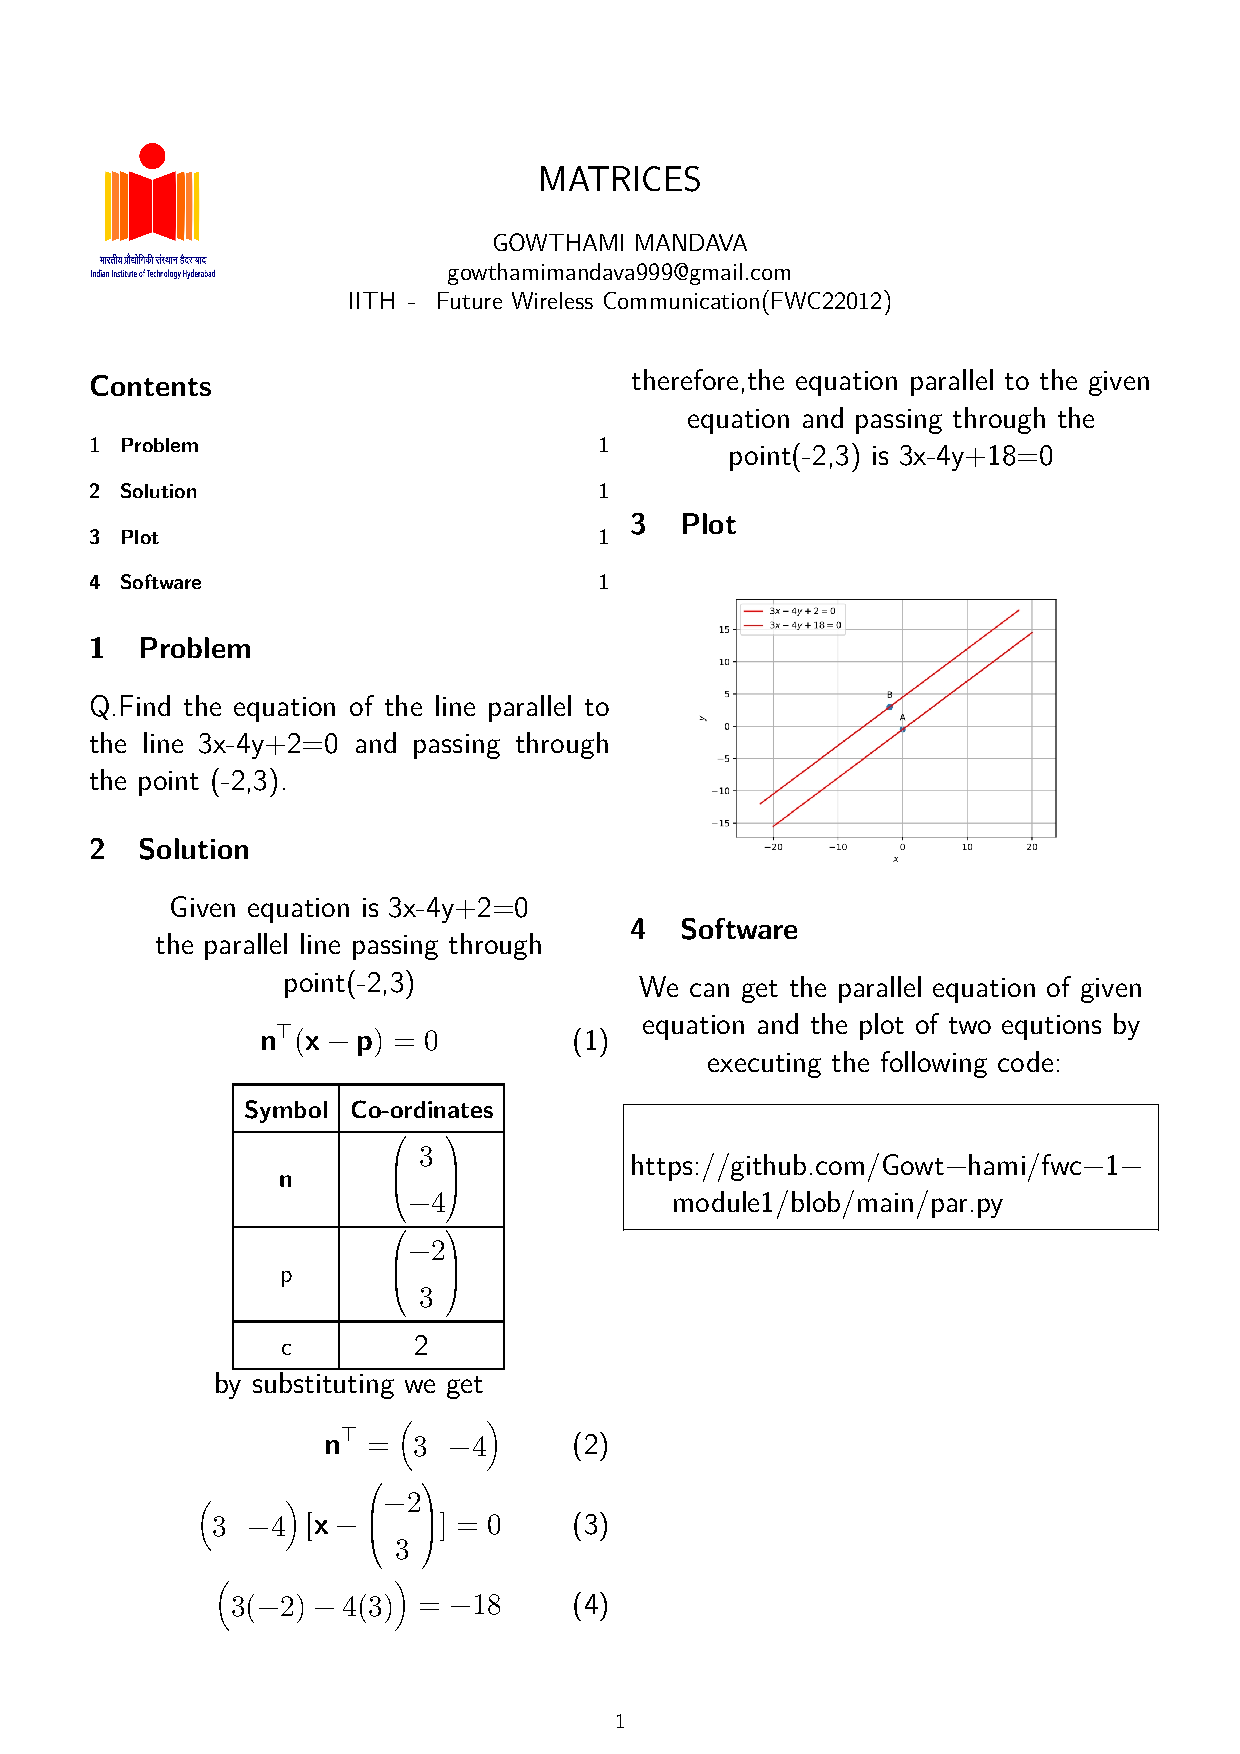
\includegraphics[scale=0.275]{mat.jpg}
  \section{Software}
  We can get the parallel equation of given equation and the plot of two equtions by executing the following code:
 \vspace{3mm} 
\begin{lstlisting}

https://github.com/Gowt-hami/fwc-1-module1/blob/main/par.py
\end{lstlisting}
\end{document}
\fi

\item 
\item 
\label{chapters/11/10/3/9}
\iffalse
\def\mytitle{LINE ASSIGNMENT}
\def\myauthor{G.Kumar}
\def\contact{kumargandhamaneni20016@gmail.com}
\def\mymodule{Future Wireless Communication (FWC)}
\documentclass[10pt, a4paper]{article}
\usepackage[a4paper,outer=1.5cm,inner=1.5cm,top=1.75cm,bottom=1.5cm]{geometry}
\twocolumn
\usepackage{graphicx}
\graphicspath{{./images/}}
\usepackage[colorlinks,linkcolor={black},citecolor={blue!80!black},urlcolor={blue!80!black}]{hyperref}
\usepackage[parfill]{parskip}
\usepackage{lmodern}
\usepackage{tikz}
\usepackage{physics}
\usepackage{tabularx}
\usetikzlibrary{calc}
\usepackage{amsmath}
\usepackage{amssymb}
\renewcommand*\familydefault{\sfdefault}
\usepackage{watermark}
\usepackage{lipsum}
\usepackage{xcolor}
\usepackage{listings}
\usepackage{float}
\usepackage{titlesec}
\providecommand{\mtx}[1]{\mathbf{#1}}
\titlespacing{\subsection}{1pt}{\parskip}{3pt}
\titlespacing{\subsubsection}{0pt}{\parskip}{-\parskip}
\titlespacing{\paragraph}{0pt}{\parskip}{\parskip}
\newcommand{\figuremacro}[5]{
    \begin{figure}[#1]
        \centering
        \includegraphics[width=#5\columnwidth]{#2}
        \caption[#3]{\textbf{#3}#4}
        \label{fig:#2}
    \end{figure}
}
\newcommand{\myvec}[1]{\ensuremath{\begin{pmatrix}#1\end{pmatrix}}}
\let\vec\mathbf
\lstset{
frame=single, 
breaklines=true,
columns=fullflexible
}
\thiswatermark{\centering \put(0,-105.0){
\includegraphics[scale=0.35]{iith}} }
\title{\mytitle}
\author{\myauthor\hspace{1em}\\\contact\\IITH\hspace{0.5em}-\hspace{0.5em}\mymodule}
\date{}
\begin{document}
	\maketitle
\section*{Problem}
\fi
   Find angle between the lines,$\sqrt{3}x+y=1$ and $x+\sqrt{3}y$=1.
   \\
   \solution 
   \iffalse
   \section*{Solution}
   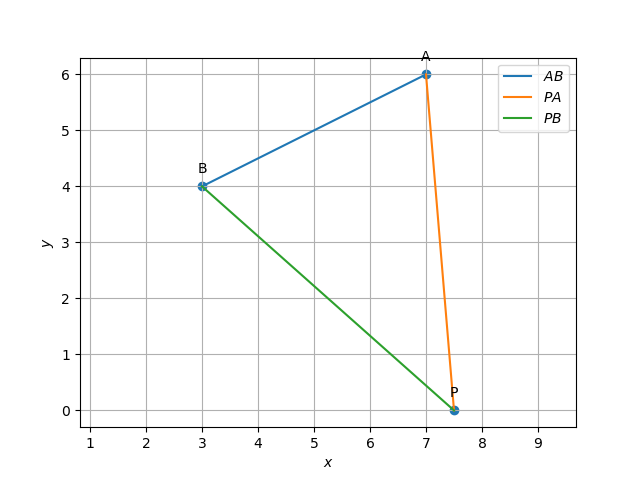
\includegraphics[scale=0.55]{line.png}
   The input parameters for this construction are :
   \begin{center}
\begin{tabular}{|c|c|c|}
	\hline
	\textbf{Symbol}&\textbf{Value}&\textbf{Description}\\
	\hline
	P&$\
	\begin{pmatrix}
		0.57736 \\
		0 \\
	\end{pmatrix}$%
	&Point P\\ 
	\hline
	X&$\
	\begin{pmatrix}
		0.36603 \\
		0.36603 \\
	\end{pmatrix}$%
	&Point X\\
	\hline
	Q&$\
	\begin{pmatrix}
		1 \\
		0 \\
	\end{pmatrix}$%
	&Point Q\\
	
	\hline
\end{tabular}
\end{center}
   \subsection*{Step 1}
   Given two equations are, \\
   \begin{equation}
   \sqrt{3}x+y=1 
   \end{equation}
   \begin{equation}
   x+\sqrt{3}y=1 
   \end{equation}
   Equation(1) in vector form is given as,
   \fi
From    the given equations, the normal vectors can be expressed as
\iffalse
   \begin{align}
   \myvec{\sqrt{3}&1}\vec{x}=1
   \end{align}
   From this, Normal vector to the line is given as,
   \fi
   \begin{align}
	   \vec{n}_1=\myvec{\sqrt{3}\\1},
	   \vec{n}_2=\myvec{1\\\sqrt{3}}
   \end{align}
   \iffalse
   So, the direction vector of the line is given as,
\begin{eqnarray*}
   \vec{m2}=\myvec{-\sqrt{3}\\1}
\end{eqnarray*}     

\subsection*{Step 2}
Now, Angle between any two lines,using their direction vectors, is given by, \\
\fi
The angle between the lines can then be expressed as
\begin{align}
	cos\theta&=\frac{\vec{n}_1^T\vec{n}_2}{\norm{\vec{n}_1}\norm{\vec{n}_2}}
	\\
	&=\frac{\sqrt{3}}{2} 
	\\
	\text{or, }
\theta=30\degree
\end{align}
\iffalse
\begin{eqnarray}
 cos\angle{x}=\frac{(\vec{m1})^T(\vec{m2})}{\norm{\vec{m1}}\norm{\vec{m2}}}\
\end{eqnarray}
\begin{eqnarray}
 cos\angle{x}=\frac{\myvec{-1\\\sqrt{3}}^T\myvec{-\sqrt{3}\\1}}{\norm{\myvec{-1\\\sqrt{3}}}\norm{\myvec{-\sqrt{3}\\1}}}
\end{eqnarray}
By solving the above equation, we get, \\
\begin{equation}
cos\angle{x}=\frac{\sqrt{3}}{2} \\
\end{equation}
This Implies,
\begin{equation*}
\angle{x}=30^\circ
\end{equation*}
Therefore, the angle between given two lines is $30^\circ$. \\
\bibliographystyle{ieeetr}
\end{document}
\fi

\item 
\item 
\item 
\item 
\item 
\item 
\item 
\item 
\item 

\end{enumerate}
